\documentclass[11pt]{article}
\usepackage{geometry}
\usepackage{graphicx}
\usepackage{epstopdf}
\usepackage{listings}
\usepackage{float}
\usepackage{csvsimple}

\begin{document}
\section{1/24/16}
\subsection{Permutation testing}
In order to test how the algorithm returns the permutation results, I set up sample matrices using \verb|create_toy.m| and recorded the distance between the result returned by the algorithm (\verb|eig_perm|) and that of the actual input data (\verb|ss|).

\lstset{language=Matlab, caption=Compare Permutations}
\begin{lstlisting}[frame=single]
rois = 33;
noise_mag = 0;
trace_type = 'sines';
shift = 10;
y = zeros(1,100);
for i = 1:length(y)
	[Z, ss] = create_toy(trace_type, 'rois', rois, ...
		'noisemag', noise_mag, ...
		'shift', shift);
	[eig_phases,eig_perm,slm,evals] = cyclic_analysis(Z);
	y(i) = cyclic_distance(ss,eig_perm);
end
plot(y)
\end{lstlisting}

The function \verb|create_toy| produces a set of \verb|rois| identical sine waves randomly spread over a \verb|shift| time step period (i.e., each copy of the trace is shifted along the x axis so that all copies are within \verb|shift| time steps of each other). The variable \verb|ss| shows the ordering of the traces produced. Using the setting above, for example, a data set like that in on the left of Figure 1 is produced. The figure on the right shows that the algorithm returns the identical permutation each time.
\begin{figure}
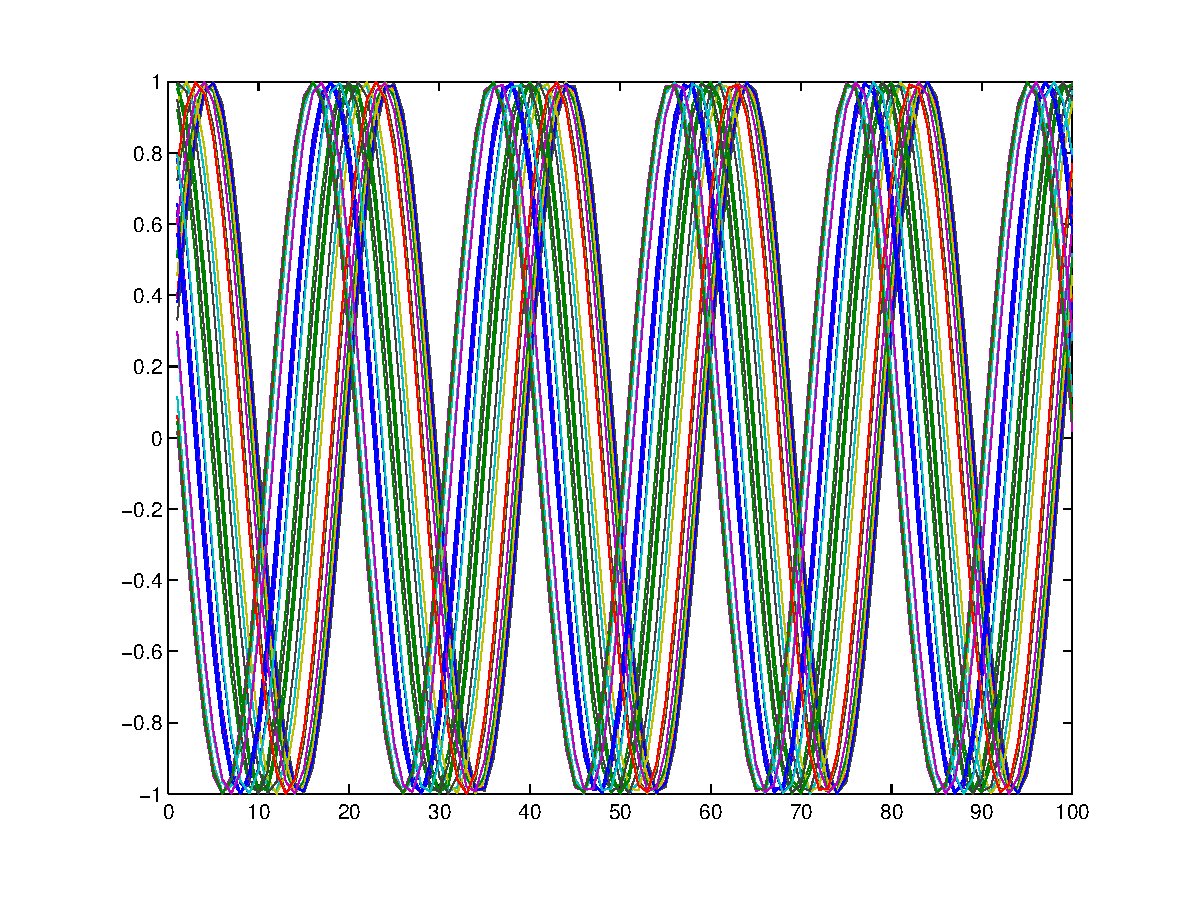
\includegraphics[width=.45\textwidth]{pictures/1_24_16/sine_toy.eps}
\includegraphics[width=.45\textwidth]{pictures/1_24_16/sine_cpsn_noNoise.eps}
\caption{Left: Sample data created from sine waves shifted randomly at most 10 time steps apart (no added noise). Right: Comparison of the permutation returned by the algorithm with that of the actual data set for 100 separately generated data sets.}
\end{figure}
The distance is measured using \verb|cyclic_distance(V1,V2)| which simply counts the how many steps V2 is from V1 (let V1 be (1:5), then [2,1,3,4,5] is a distance of 1 from V1 and [2,3,4,5,1] is a distance of 5 from V1.) This doesn't really count "cyclic distance" but works for this application since we would like to see if we are picking up the correct starting point and cycling in the right direction. 
Increasing \verb|shift| to 18 (the period for the sine wave is 20) starts to mess up the permutation since the algorithm can't determine the proper starting point.
\begin{figure}[H]
\includegraphics[width=.45\textwidth]{pictures/1_24_16/sine_cpsn_shift18.eps}
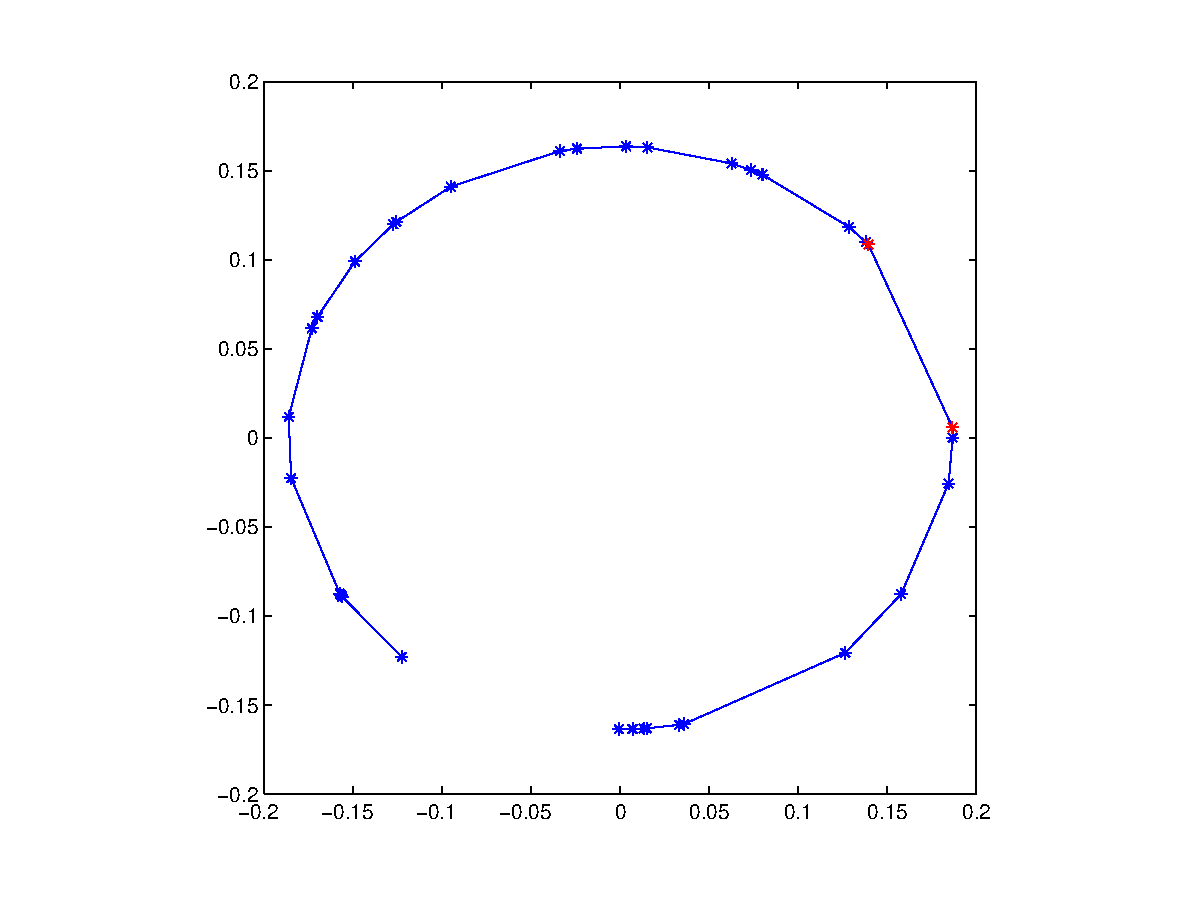
\includegraphics[width=.45\textwidth]{pictures/1_24_16/phases_shift18.eps}
\caption{Left: Algorithm performance when \texttt shift=18. Right: Plot of phases for a permutation which the algorithm had shifted by 11 places (distance = 242). The red asterisks highlight the 11th and 12th points in the cycle.}  
\end{figure}
The algorithm determines the starting point by finding the largest gap between points in the phase plot (greatest difference in angle). Once the phases are too spread out, the largest gap can easily be between a pair of middle points. Note, however, that still the algorithm cycles in the correct direction in each case. 


\section{Listings}
\lstset{language=Matlab, caption=cyclic\_distance}
\begin{lstlisting}[frame=single]
function [dist] = cyclic_distance(V1, V2)
[~, ss] = sort([V1(:), V2(:)]);
dist = sum(abs(diff(ss,1,2)))/2;
\end{lstlisting}

\subsection{Movies}
\subsubsection{Data Treatment}
In the original data set, there are gaps in the data for some genres and not all genres began at the same time so some initial data treatment was required. First, years in which there were gaps in the data were inpainted using linear interpolation. Next, the genre counts were taken on a log scale to account for the fact that movie production has grown exponentially. Finally, only years in which genres had data points were considered (1916-2015). The film-noir genre had to be excluded since the production years were so limited.
The following table shows the results of \verb|analyze_cyclicity| on the movie data (processed as described above). 
\begin{figure}[H]
\begin{minipage}{.3\textwidth}
\csvautotabular{tables/genre_results.txt}
\end{minipage}
\hfill
\begin{minipage}{.65\textwidth}
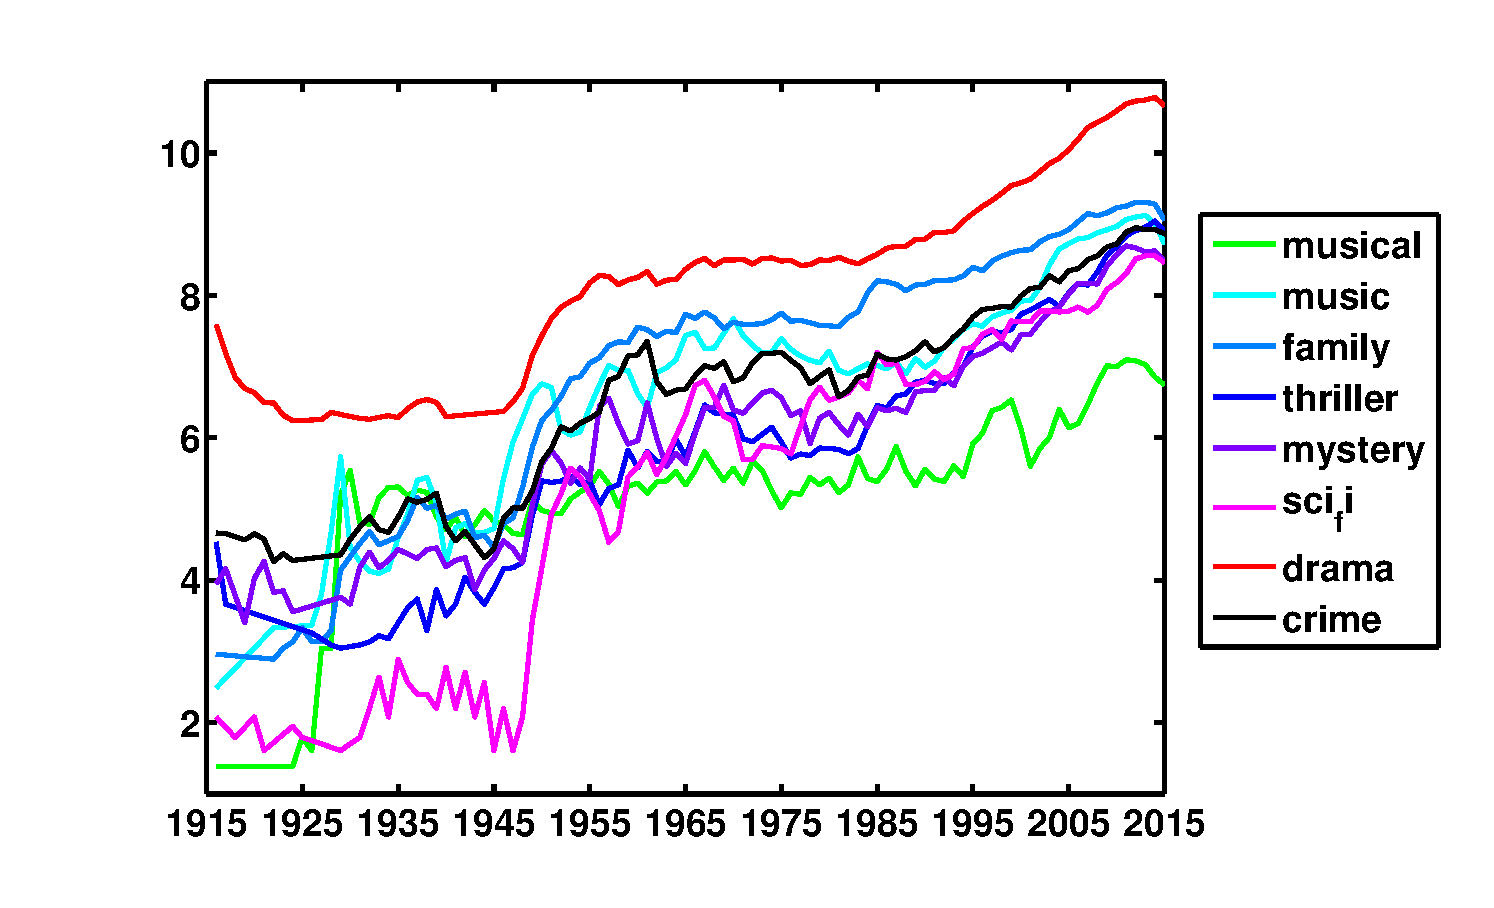
\includegraphics[width=\textwidth]{pictures/movie_data_all_yrs.eps}
\caption{Traces from the first eight genres.}
\end{minipage}
\end{figure}
\begin{figure}[H]
\centering
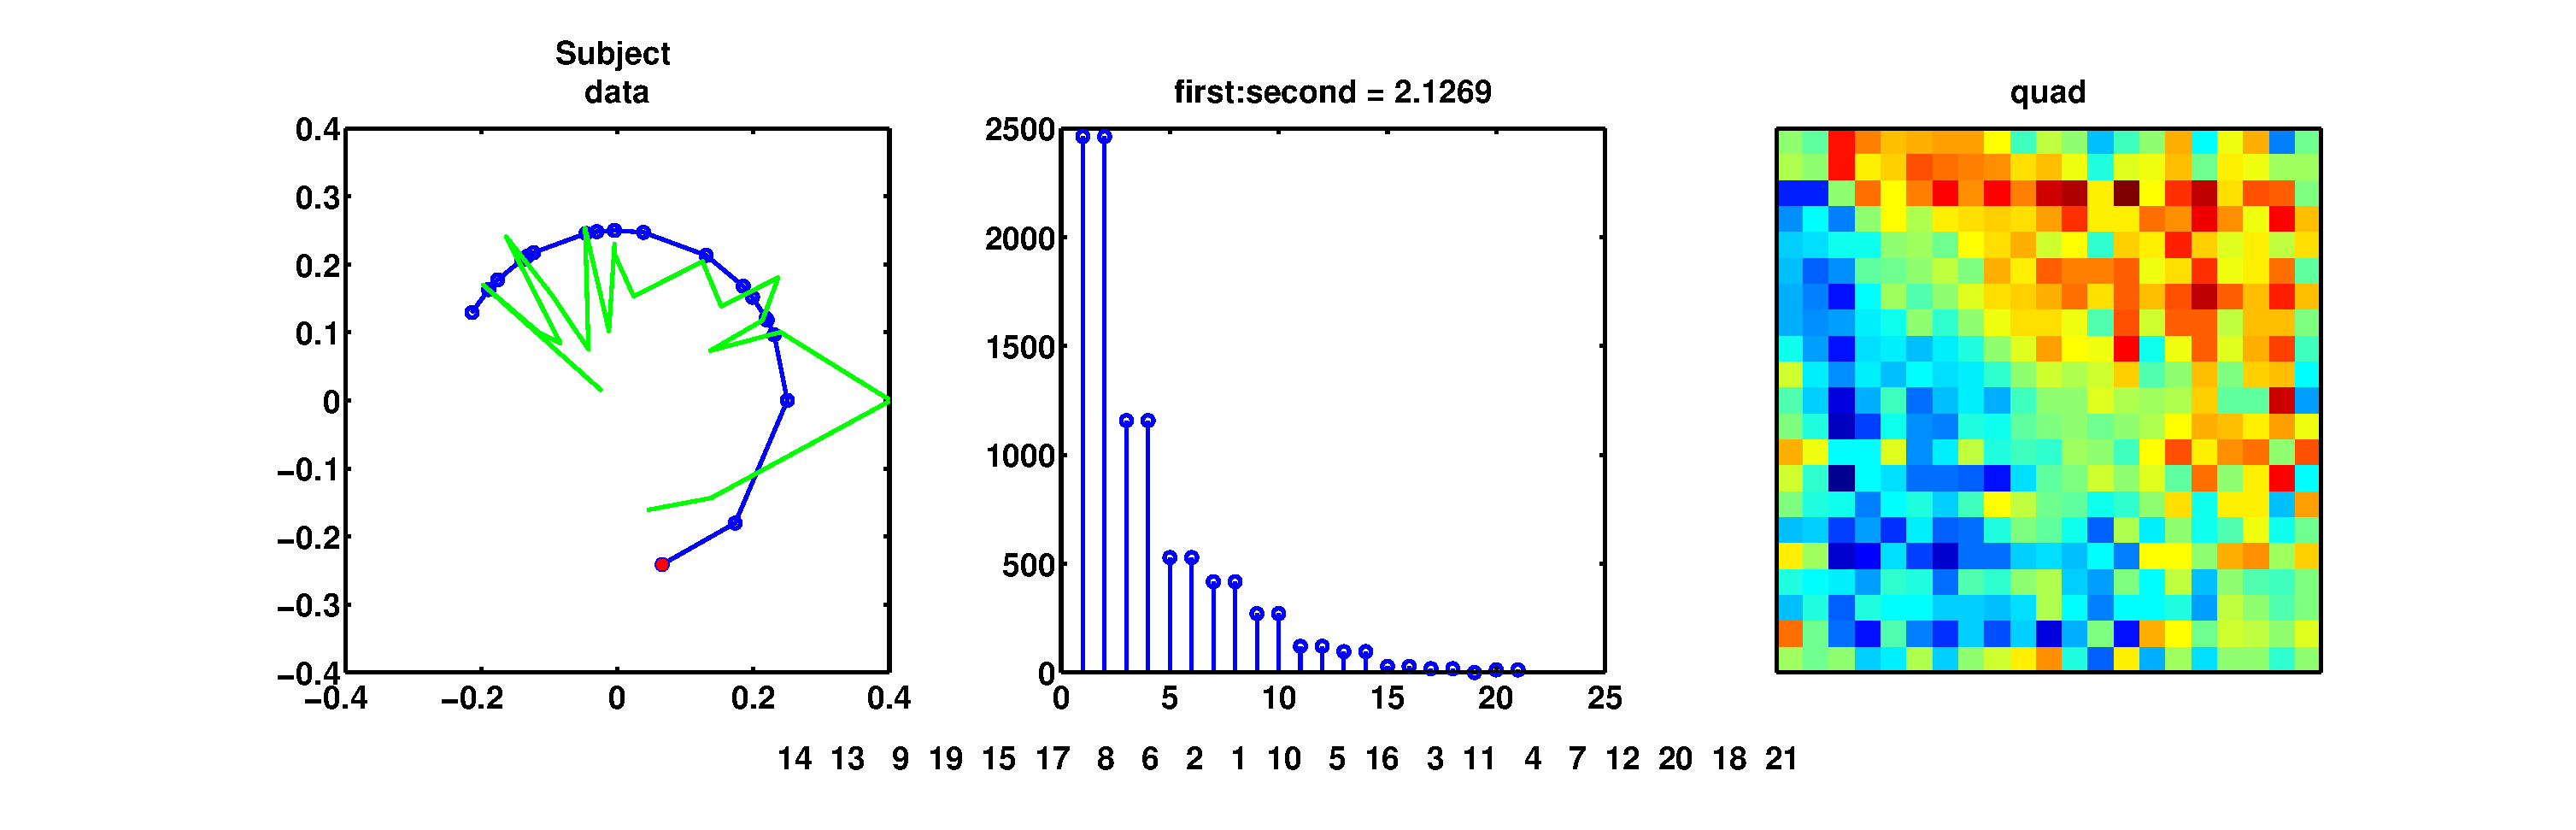
\includegraphics[trim= 130 0 130 0, clip, width=\textwidth]{pictures/movie_data_QC.eps}
\caption{Cyclicity results using quadratic variation normalization}
\end{figure}
Note that the Musicals and Music genres look very similar to each other, but dissimilar to everything else and show a drastic jump around 1925. Since this is such a long time ago, it seemed worth considering more recent trends in the data.
\begin{figure}[H]
\begin{minipage}{.3\textwidth}
\csvautotabular{../Movies/Recent_data/Results/genre_results_table.txt}
\end{minipage}
\hfill
\begin{minipage}{.6\textwidth}
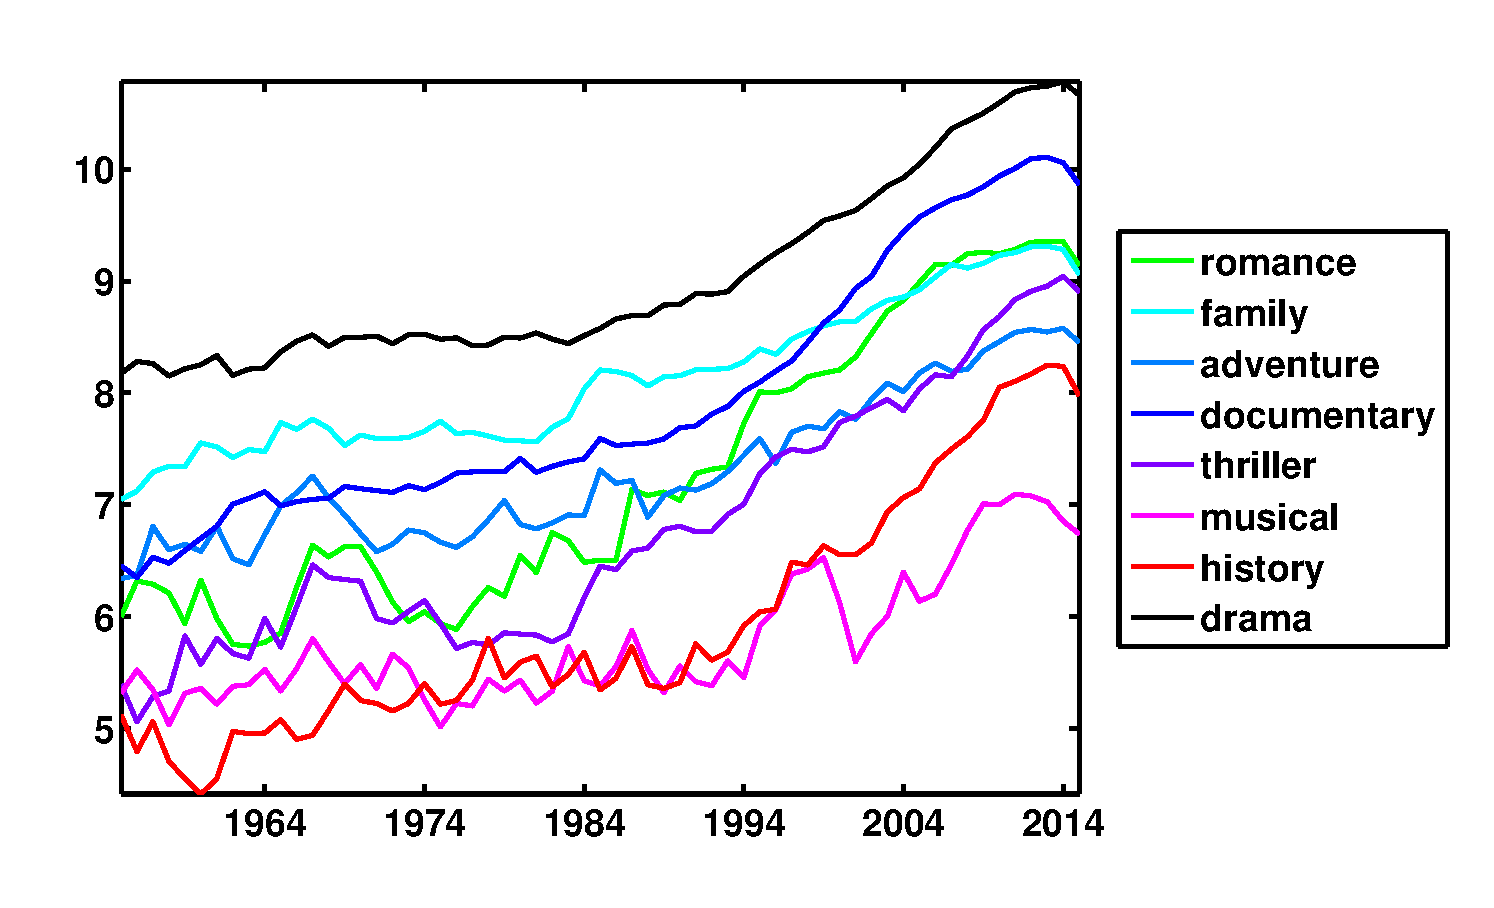
\includegraphics[width=\textwidth]{pictures/movie_data_1955-2015.eps}
\caption{Traces from the first eight genres using only years 1955-2015 in the cyclicity calculation.}
\end{minipage}
\end{figure}
\begin{figure}[H]
\centering
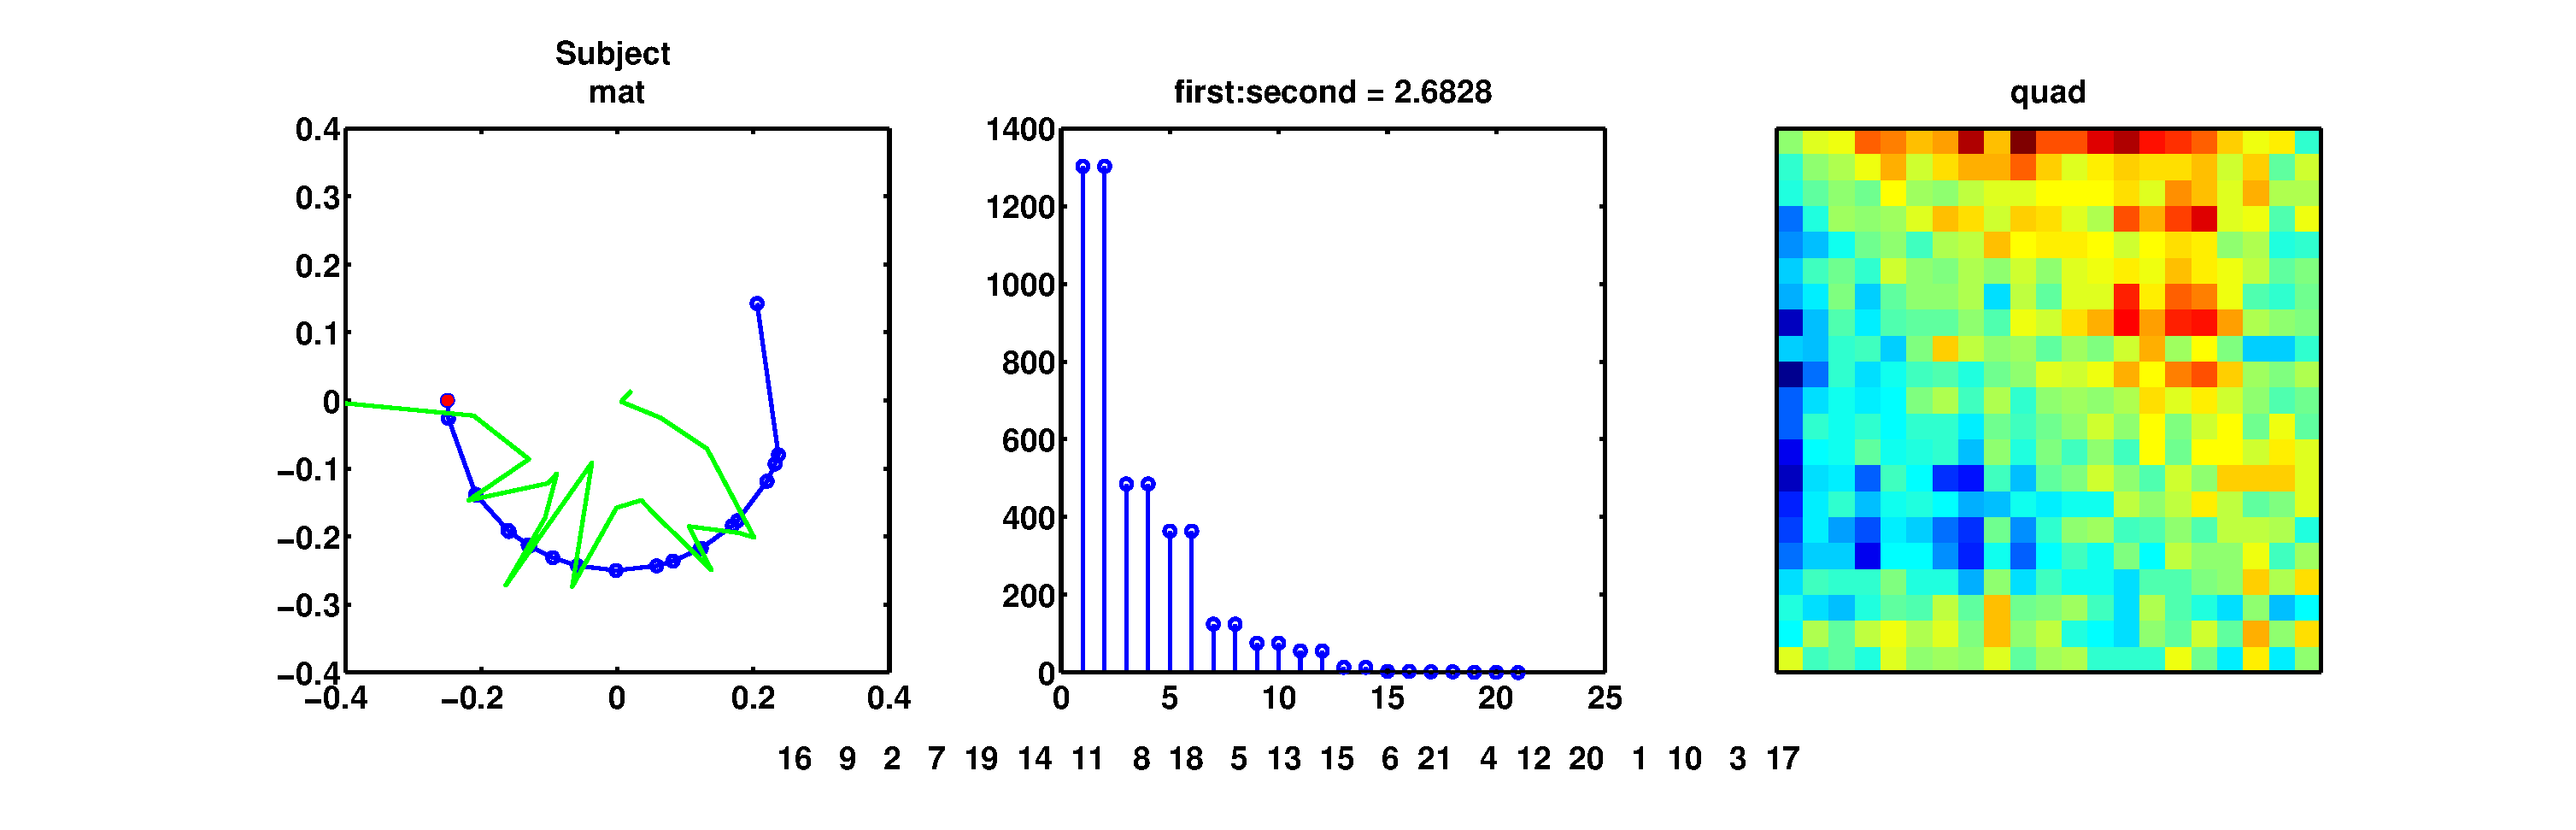
\includegraphics[trim= 130 0 130 0, clip, width=\textwidth]{pictures/movie_data_1955-2015_QC.eps}
\caption{Cyclicity results from 1955-2015 movie data using quadratic variation normalization}
\end{figure}


\end{document}